\documentclass[compress]{beamer}
\usepackage{epstopdf}
\usepackage{graphicx}
\usepackage{lmodern}
\usepackage{tikz}
\usepackage{verbatim}

\usetikzlibrary{decorations.pathreplacing,calc}

\newcommand{\tikzmark}[2][-3pt]{\tikz[remember picture, overlay, baseline=-2.0ex]\node[#1](#2){};}

\tikzset{brace/.style={decorate, decoration={brace}},
 brace mirrored/.style={decorate, decoration={brace,mirror}},
}

\newcounter{brace}
\setcounter{brace}{0}
\newcommand{\drawbrace}[3][brace]{%
 \refstepcounter{brace}
  \tikz[remember picture, overlay]\draw[#1] (#2.center)--(#3.center)node[pos=0.5, name=brace-\thebrace]{};
}

\newcounter{arrow}
\setcounter{arrow}{0}
\newcommand{\drawcurvedarrow}[3][]{%
 \refstepcounter{arrow}
  \tikz[remember picture, overlay]\draw (#2.center)edge[#1]node[coordinate,pos=0.5, name=arrow-\thearrow]{}(#3.center);
}

% #1 options, #2 position, #3 text 
\newcommand{\annote}[3][]{%
 \tikz[remember picture, overlay]\node[#1] at (#2) {#3};
}

\renewcommand*\footnoterule{} % remove footnote rule

\definecolor{emerald}{RGB}{0,166,79}

% Load the usyd template
% Template from https://bitbucket.org/silvo/usyd-beamer-template

% Include this file with % Template from https://bitbucket.org/silvo/usyd-beamer-template

% Include this file with % Template from https://bitbucket.org/silvo/usyd-beamer-template

% Include this file with \input{usyd-beamer.tex}

\usetheme{default}

% Turn off navigation bar:
\beamertemplatenavigationsymbolsempty

% Colours:
%\definecolor{sydneyred}{RGB}{206,17,38}
\definecolor{sydneyred}{RGB}{240,17,38}
\setbeamercolor{frametitle}{fg=black}
\setbeamercolor{structure}{fg=sydneyred}
\setbeamercolor{section in head/foot}{fg=black}

\defbeamertemplate*{footline}{usyd}
{%
	\begin{beamercolorbox}[ht=2.25ex,dp=3.75ex,center]{section in head/foot}
		\insertnavigation{0.99\paperwidth}
	\end{beamercolorbox}%
}%

% Default slide background:
\usebackgroundtemplate{\includegraphics[width=\paperwidth,height=\paperheight]{usyd-beamer/normalslide.png}}

% Macro for indenting a paragraph
% Usage: \begin{leftindent}{20mm} paragraph \\ goes \\ here \end{leftindent}
\newenvironment{leftindent}[1] { %
	\begin{list}{}{ %
		\setlength{\leftmargin}{#1} %
	} %
	\item[] %
} { %
	\end{list} %
}


% Move frame title to right hand side
\setbeamertemplate{frametitle}{ %
	\vspace{4mm}
   	\hbox{ %
   		\begin{beamercolorbox}[wd=\paperwidth]{frametitle}%
  	    	\hfill \insertframetitle \hspace{9mm} %
   		\end{beamercolorbox} %
   		\vspace{4mm} % we don't want the main text overlapping the image
   	} %
}

% Macro for including a title slide
% Usage: \usydtitleframe{Title}{Subtitle}{Author info} 
\newcommand{\usydtitleframe}[3] {{ %
	\usebackgroundtemplate{\includegraphics[width=\paperwidth,height=\paperheight]{usyd-beamer/titleslide.png}} %
	\begin{frame}[t,plain]{} %
		\vspace{10mm} %
		\begin{leftindent}{10mm} %
			{\LARGE #1 } \\ %
			\vspace{3mm} %
			{\large #2 } %
		\end{leftindent} %
    \vskip3cm
    \begin{beamercolorbox}[left,leftskip=4ex]{}
      {\scriptsize FACULTY OF\\ENGINEERING \&\\INFORMATION\\TECHNOLOGIES}
    \end{beamercolorbox}
    \vskip-13pt
    \begin{beamercolorbox}[right,rightskip=-4ex]{} %
      {\small #3} %
    \end{beamercolorbox} %
	\end{frame} %
}}

\newcommand{\group}[1]{\section{#1}\subsection{}}
\renewcommand{\emph}[1]{\alert{#1}}


\usetheme{default}

% Turn off navigation bar:
\beamertemplatenavigationsymbolsempty

% Colours:
%\definecolor{sydneyred}{RGB}{206,17,38}
\definecolor{sydneyred}{RGB}{240,17,38}
\setbeamercolor{frametitle}{fg=black}
\setbeamercolor{structure}{fg=sydneyred}
\setbeamercolor{section in head/foot}{fg=black}

\defbeamertemplate*{footline}{usyd}
{%
	\begin{beamercolorbox}[ht=2.25ex,dp=3.75ex,center]{section in head/foot}
		\insertnavigation{0.99\paperwidth}
	\end{beamercolorbox}%
}%

% Default slide background:
\usebackgroundtemplate{\includegraphics[width=\paperwidth,height=\paperheight]{usyd-beamer/normalslide.png}}

% Macro for indenting a paragraph
% Usage: \begin{leftindent}{20mm} paragraph \\ goes \\ here \end{leftindent}
\newenvironment{leftindent}[1] { %
	\begin{list}{}{ %
		\setlength{\leftmargin}{#1} %
	} %
	\item[] %
} { %
	\end{list} %
}


% Move frame title to right hand side
\setbeamertemplate{frametitle}{ %
	\vspace{4mm}
   	\hbox{ %
   		\begin{beamercolorbox}[wd=\paperwidth]{frametitle}%
  	    	\hfill \insertframetitle \hspace{9mm} %
   		\end{beamercolorbox} %
   		\vspace{4mm} % we don't want the main text overlapping the image
   	} %
}

% Macro for including a title slide
% Usage: \usydtitleframe{Title}{Subtitle}{Author info} 
\newcommand{\usydtitleframe}[3] {{ %
	\usebackgroundtemplate{\includegraphics[width=\paperwidth,height=\paperheight]{usyd-beamer/titleslide.png}} %
	\begin{frame}[t,plain]{} %
		\vspace{10mm} %
		\begin{leftindent}{10mm} %
			{\LARGE #1 } \\ %
			\vspace{3mm} %
			{\large #2 } %
		\end{leftindent} %
    \vskip3cm
    \begin{beamercolorbox}[left,leftskip=4ex]{}
      {\scriptsize FACULTY OF\\ENGINEERING \&\\INFORMATION\\TECHNOLOGIES}
    \end{beamercolorbox}
    \vskip-13pt
    \begin{beamercolorbox}[right,rightskip=-4ex]{} %
      {\small #3} %
    \end{beamercolorbox} %
	\end{frame} %
}}

\newcommand{\group}[1]{\section{#1}\subsection{}}
\renewcommand{\emph}[1]{\alert{#1}}


\usetheme{default}

% Turn off navigation bar:
\beamertemplatenavigationsymbolsempty

% Colours:
%\definecolor{sydneyred}{RGB}{206,17,38}
\definecolor{sydneyred}{RGB}{240,17,38}
\setbeamercolor{frametitle}{fg=black}
\setbeamercolor{structure}{fg=sydneyred}
\setbeamercolor{section in head/foot}{fg=black}

\defbeamertemplate*{footline}{usyd}
{%
	\begin{beamercolorbox}[ht=2.25ex,dp=3.75ex,center]{section in head/foot}
		\insertnavigation{0.99\paperwidth}
	\end{beamercolorbox}%
}%

% Default slide background:
\usebackgroundtemplate{\includegraphics[width=\paperwidth,height=\paperheight]{usyd-beamer/normalslide.png}}

% Macro for indenting a paragraph
% Usage: \begin{leftindent}{20mm} paragraph \\ goes \\ here \end{leftindent}
\newenvironment{leftindent}[1] { %
	\begin{list}{}{ %
		\setlength{\leftmargin}{#1} %
	} %
	\item[] %
} { %
	\end{list} %
}


% Move frame title to right hand side
\setbeamertemplate{frametitle}{ %
	\vspace{4mm}
   	\hbox{ %
   		\begin{beamercolorbox}[wd=\paperwidth]{frametitle}%
  	    	\hfill \insertframetitle \hspace{9mm} %
   		\end{beamercolorbox} %
   		\vspace{4mm} % we don't want the main text overlapping the image
   	} %
}

% Macro for including a title slide
% Usage: \usydtitleframe{Title}{Subtitle}{Author info} 
\newcommand{\usydtitleframe}[3] {{ %
	\usebackgroundtemplate{\includegraphics[width=\paperwidth,height=\paperheight]{usyd-beamer/titleslide.png}} %
	\begin{frame}[t,plain]{} %
		\vspace{10mm} %
		\begin{leftindent}{10mm} %
			{\LARGE #1 } \\ %
			\vspace{3mm} %
			{\large #2 } %
		\end{leftindent} %
    \vskip3cm
    \begin{beamercolorbox}[left,leftskip=4ex]{}
      {\scriptsize FACULTY OF\\ENGINEERING \&\\INFORMATION\\TECHNOLOGIES}
    \end{beamercolorbox}
    \vskip-13pt
    \begin{beamercolorbox}[right,rightskip=-4ex]{} %
      {\small #3} %
    \end{beamercolorbox} %
	\end{frame} %
}}

\newcommand{\group}[1]{\section{#1}\subsection{}}
\renewcommand{\emph}[1]{\alert{#1}}


\setbeamerfont{footnote}{size=\tiny}

\begin{document}
\usydtitleframe{Data Mining Methods for Predicting Length of Hospital Stay}{}{\textbf{Tianyu Pu} Honours Student \\
  Supervisor: Irena Koprinska}

\section{Introduction}
\subsection{}
\begin{frame}{Introduction}
Imagine that you have just been admitted to hospital...
  \pause

\vspace{0.5cm}
\textbf{Why do we care?}
\end{frame}

\subsection{}
\begin{frame}{Outline of talk}
The problem

\vspace{0.5cm}
Background and previous work

\vspace{0.5cm}
Our approach

\vspace{0.5cm}
Results and discussion

\vspace{0.5cm}
Conclusions and future work
\end{frame}

\section{The Problem}
\subsection{}
\begin{frame}{The problem}
Given
\begin{center}
\begin{tabular}{cccc|c}
\tikzmark[]{x}age & gender & heart rate & ... & length of stay (LOS)\tikzmark[]{y} \\
\hline
\tikzmark[xshift=-0.80ex, yshift=-1ex]{a}45 & F & 122 & ... & $>$ 2 days \\
23 & M & 98 & ... & $\leq$ 2 days \\
\multicolumn{4}{c|}{\tikzmark[xshift=-13.3ex, yshift=-2ex]{b}...} & ... \\
\end{tabular}
\end{center}
\drawbrace[brace mirrored, thick, gray]{y}{x}
\drawbrace[brace mirrored, thick, gray]{a}{b}
\annote[yshift=1.5ex, gray]{brace-1}{\scriptsize features}
\annote[left, gray]{brace-2}{\scriptsize examples}

\vspace{0.5cm}
Predict LOS category for new patient
\begin{center}
\begin{tabular}{cccc|c}
age & gender & heart rate & ... & length of stay (LOS)  \\
\hline
34 & F & 101 & ... & ? \\
\end{tabular}
\end{center}
\end{frame}

\section{Background and Previous Work}
\subsection{}
\begin{frame}{Prediction}
\begin{center}
\includegraphics<1>{learning.pdf}
\includegraphics<2>{learning-focus2.pdf}
\end{center}
\end{frame}

\subsection{}
\begin{frame}{Feature discretisation and selection}
\textbf{Discretisation}
\begin{itemize}
\item Convert numeric features into categorical features
\item \textit{Supervised} discretisation
\item Why?
\end{itemize}

\vspace{0.5cm}

  \pause
\textbf{Selection}
\begin{itemize}
\item Find a subset of features that are the most `relevant'
\item Two ways: \textit{manual} and \textit{automatic}
\item Why?
\end{itemize}
\end{frame}

\subsection{}
\begin{frame}{Learning algorithms}
\textbf{Logistic regression}

One of the most widely used approaches in LOS prediction
\begin{equation*}
\begin{aligned}
\text{log}\left(\dfrac{\text{probability of LOS}\leq\text{2 days}}{\text{probability of LOS}>\text{2 days}}\right) &= b_0 + b_1\text{age} + b_2\text{gender} + \ldots
\end{aligned}
\end{equation*}
  \pause

\textbf{Others}

Artificial neural networks, ...
\end{frame}

\section{Approach}
\subsection{}
\begin{frame}{Proposed approach (1)}
Store all examples and do not try to generalise

Classify new example by looking at $k$ most `similar' (`nearest') examples
\begin{itemize}
\item \textit{Nearest neighbour} approach
\end{itemize}

\vspace{0.5cm}
\textbf{Similarity}

Typical approach: \textit{Euclidean distance}

\begin{equation*}
\sqrt{(x_1-y_1)^2 + (x_2-y_2)^2 + \ldots}
\end{equation*}
\end{frame}

\subsection{}
\begin{frame}{Proposed approach (2)}
Our approach: \textit{Ranked distance}
\begin{equation*}
w_1|x_1-y_1| + w_2|x_2-y_2| + \ldots
\end{equation*}

\vspace{0.5cm}
\textbf{Intuition}

The relative importance of a feature should determine its contribution to the similarity
\end{frame}

\subsection{}
\begin{frame}{Evaluation}
\textbf{Two datasets}: trauma and general hospital LOS data

\vspace{0.5cm}

\textbf{Procedure}:
\begin{enumerate}
\item Preprocess and discretise datasets $\implies$ 4 sets of data
\item Systematically evaluate 11 learning algorithms with 5 \textit{automatic} and 2 \textit{manual} feature selection methods
\end{enumerate}

\vspace{0.5cm}

  \pause
\textbf{Performance measures}: \textit{accuracy} and \textit{area under the curve (AUC)}
\end{frame}

\section{Results}
\subsection{}
\begin{frame}{Summary of best results}
\textbf{Trauma dataset}
\begin{center}
\begin{tabular}{l|cc}
 & Baseline & Our best result \\
\hline
Accuracy (\%) & 75.06 (19) & \textcolor{emerald}{77.81} (\textcolor{emerald}{11})\footnote{1-NN, C4.5 wrapper, discretised} \\
AUC & 0.812 (19) & \textcolor{emerald}{0.846} (\textcolor{sydneyred}{29})\footnote{Logistic regression, no feature selection, discretised} \\
\end{tabular}
\end{center}

\pause
\textbf{General hospital dataset}
\begin{center}
\begin{tabular}{l|c}
 & Our best result \\
\hline
Accuracy (\%) & 98.23 (14)\footnote{C4.5 decision tree, no feature selection or discretisation} \\
AUC & 0.994 (14)\footnote{Logistic regression, SVM and K*, no feature selection or discretisation} \\
\end{tabular}
\end{center}
\end{frame}

\subsection{}
\begin{frame}{Trauma data set}
\begin{center}
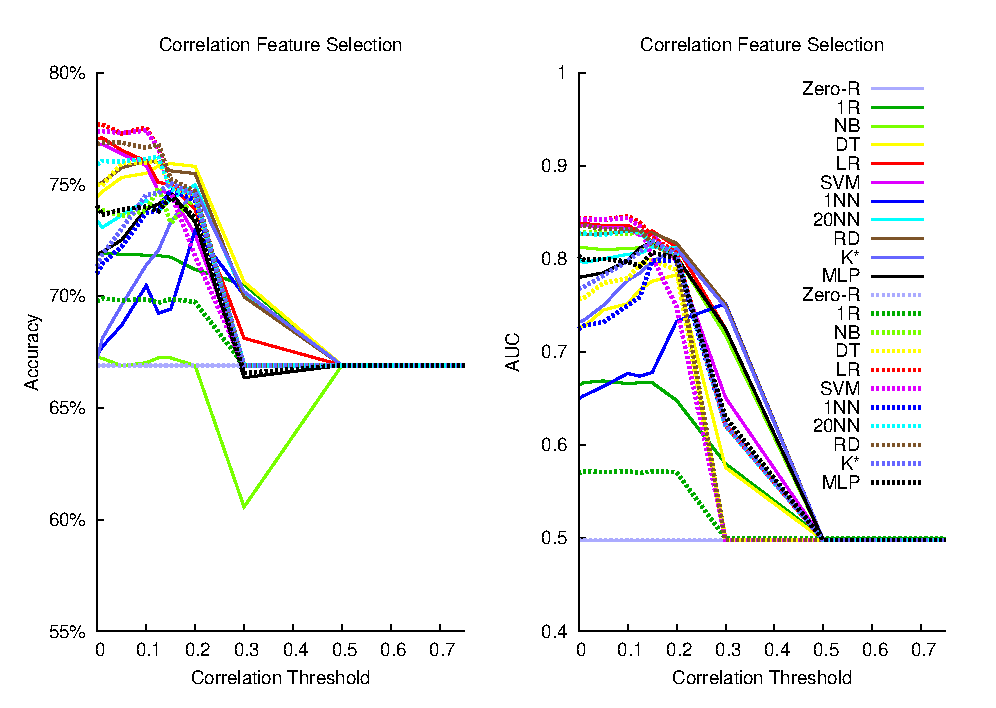
\includegraphics[width=0.93\textwidth]{tr-corr.eps}
\end{center}
\end{frame}

\subsection{}
\begin{frame}{General hospital data set}
\begin{center}
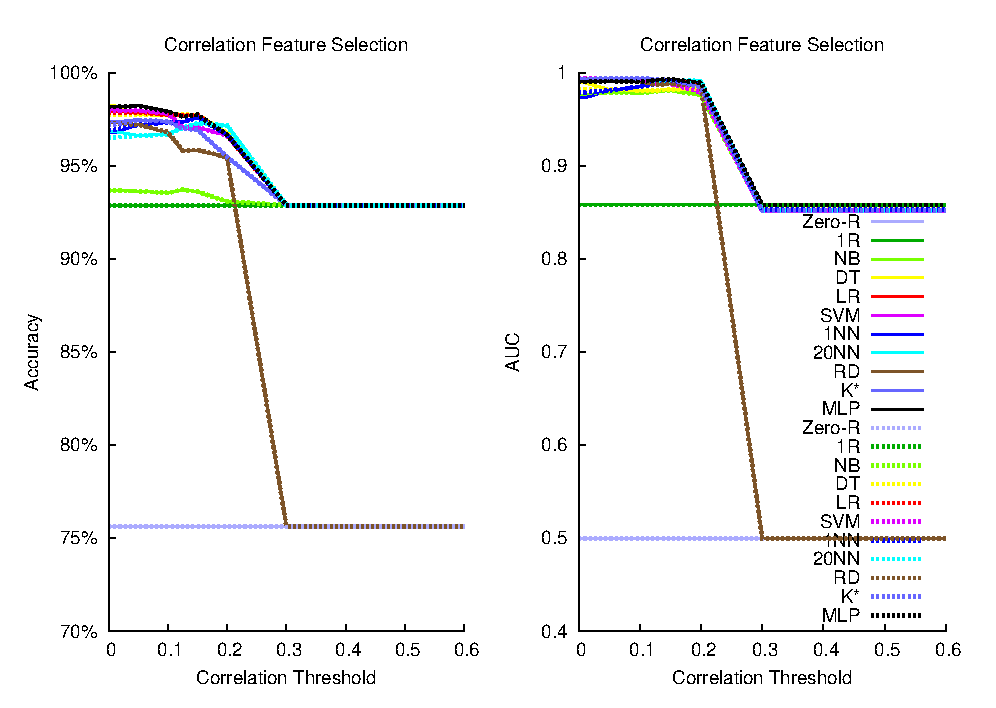
\includegraphics[width=0.92\textwidth]{pt-corr.eps}
\end{center}
\end{frame}

\subsection{}
\begin{frame}{Discussion}
Limitations of nearest neighbour methods

\vspace{0.5cm}
Trade-off between predictive power and number of features

\vspace{0.5cm}
Know your data!
\end{frame}

\section{Conclusions}
\subsection{}
\begin{frame}{Conclusions}
Comprehensive and systematic evaluation

\vspace{0.5cm}
Proposed new nearest neighbour algorithm

\vspace{0.5cm}
Improved accuracy by 2.75\% and AUC by 0.034 on the same dataset using nearest neighbour methods

\pause
\vspace{0.5cm}
\textbf{Future work}
\begin{itemize}
\item Ensembles
\item Different similarity measures
\item Implementation for doctors
\end{itemize}
\end{frame}

\end{document}
